% !TEX TS-program = lualatex
% !BIB TS-program = biber
%\documentclass[handout]{beamer}
\documentclass{beamer}
\input{../common/misomva}
\newcommand{\misoclasstinytitleslide}{Partially based on material by:  Branislav Kveton, \\[-1em] 
Mikhail Belkin, Jerry Zhu}
\newcommand{\misoclassdate}{}
\begin{document}
% Topic-specific title slide

\newcommand{\topictitle}{Online SSL: Graph Quantization}

\newcommand{\topicsubtitle}{Charikar's Algorithm and Multiplicities}
\renewcommand{\misoclasstinytitleslide}{Partially based on material by:  Branislav Kveton, \\[-1em] Mikhail Belkin, Jerry Zhu}
% Constants
\newcommand{\Rmultiplier}{R}             % Multiplier constant (typically R)

\MakeTopicSlide

\begin{frame}
\frametitle{Online SSL with Graphs: \emphcol{Graph Quantization}}
\alert{An} idea: incremental $k$-centers 
\moveb
\pause
Doubling algorithm of Charikar et al.~\cite{charikar1997incremental} 
\moveb
\pause
Keeps up to $k$ centers $C_t = \set{\bc_1, \bc_2, \dots}$ with
\moveb
\pause
\begin{itemize}[<+-| alert@+>]
 \item Distance $\bc_i, \bc_j \in C_t$  is at least $\geq R$
 \item For each new $\bx_t$,  distance to some $\bc_i \in C_t$ is less than $R$. 
 \item $|C_t|\leq k$
 \item if not possible, $R$ is doubled
\end{itemize}

\end{frame}
%%%%%%%%%%%%%%%%%%%%%%%%%%%%%%%%%%%%%%%%%%%%%%%%%%%%%%%%%%%%
\begin{frame}
\frametitle{Online SSL with Graphs: \emphcol{Graph Quantization}}

\includegraphics<1-2>[height=0.65\textheight]{../img/s3}%
\includegraphics<2>[height=0.65\textheight]{../img/s4}%
\includegraphics<3-4>[height=0.65\textheight]{../img/s5}%
\includegraphics<4>[height=0.65\textheight]{../img/s6}%
\includegraphics<5-6>[height=0.65\textheight]{../img/s7}%
\includegraphics<6>[height=0.65\textheight]{../img/s8}%

\end{frame}
%%%%%%%%%%%%%%%%%%%%%%%%%%%%%%%%%%%%%%%%%%%%%%%%%%%%%%%%%%%%
\begin{frame}
\frametitle{Online SSL with Graphs: \emphcol{Graph Quantization}}
\vspace{-0.7em}
% \textbf{How to quantize $G$?}\moveb \pause
\renewcommand{\ng}{k}
\begin{algorithm}[H]
\begin{algorithmic}[1]
{\small
%      {\bf Inputs:} \\
     \STATE  an unlabeled $\bx_t$, a set of centroids $C_{t - 1}$, multiplicities $\bv_{t - 1}$ \pause
%     {\bf Algorithm:} \\
    \IF{$(\abs{C_{t - 1}} = \ng + 1)$} 
    \STATE  $R \gets m R$ 
    \STATE \pause greedily repartition $C_{t - 1}$ into $C_t$ such that: 
    \STATE  \quad no two vertices in $C_t$ are closer than $R$ 
     \STATE \quad  for any $\bc_i \in C_{t - 1}$ exists $\bc_j \in C_t$ such that $d(\bc_i, \bc_j) < R$ 
     \STATE  \pause update $\bv_t$ to reflect the new partitioning 
    \ELSE
     \STATE  $C_t \gets C_{t - 1}$ 
     \STATE  $\bv_t \gets \bv_{t - 1}$ \pause
    \ENDIF
    \IF{$\bx_t$ is closer than $R$ to any $\bc_i \in C_t$} 
    \STATE  $\bv_t(i) \gets \bv_t(i) + 1$ 
    \ELSE 
    \STATE \pause $\bv_t(\abs{C_t} + 1) \gets 1$     
    \ENDIF
}
\end{algorithmic}
  \caption*{Online $k$-centers}
\end{algorithm}
\end{frame}
%%%%%%%%%%%%%%%%%%%%%%%%%%%%%%%%%%%%%%%%%%%%%%%%%%%%%%%%%%%%
\begin{frame}
\frametitle{Online SSL with Graphs: \emphcol{Graph Quantization}}

Doubling algorithm~\cite{charikar1997incremental} 
\moveb
\pause
To reduce growth of  $R$, we use $R \gets \Rmultiplier\times R$, with $\Rmultiplier\geq 1$
\moveb
\pause

$C_t$ is changing. \questionbox{How far can $\bx$ be from some $\bc$?}
\pause

\begin{displaymath}
R  \pause + \frac{R}{\Rmultiplier} \pause + \frac{R}{\Rmultiplier^2} \pause + \cdots 
= R\left(1 + \frac{1}{\Rmultiplier} + \frac{1}{\Rmultiplier^2} + \cdots \right) \pause 
=  \frac{R\Rmultiplier}{\Rmultiplier-1}	
\end{displaymath}

\pause
Guarantees\pause: 8-approximation algorithm.
\pause
\rightquestionbox{Why not incremental $k$-means?}

\end{frame}
%%%%%%%%%%%%%%%%%%%%%%%%%%%%%%%%%%%%%%%%%%%%%%%%%%%%%%%%%%%%

%%%%%%%%%%%%%%%%%%%%%%%%%%%%%%%%%%%%%%%%%%%%%%%%%%%%%%%%%%%%
\begin{frame}
\frametitle{Online SSL with Graphs}

\textbf{Video examples}
\moveb
{\small
\url{http://www.bkveton.com/videos/Coffee.mp4}
\moveb
\url{http://www.bkveton.com/videos/Ad.mp4}
\moveb
\url{https://misovalko.github.io/publications/kveton2009nipsdemo.adaptation.mov}
\moveb
\url{https://misovalko.github.io/publications/kveton2009nipsdemo.officespace.mov}
\moveb
%\notecol{
\tiny \url{https://misovalko.github.io/publications/press-intel-2015.mp4}%}
}
\end{frame}
%%%%%%%%%%%%%%%%%%%%%%%%%%%%%%%%%%%%%%%%%%%%%%%%%%%%%%%%%%%%
\begin{frame}
\frametitle{SSL with Graphs: Some experimental results}

\begin{center}
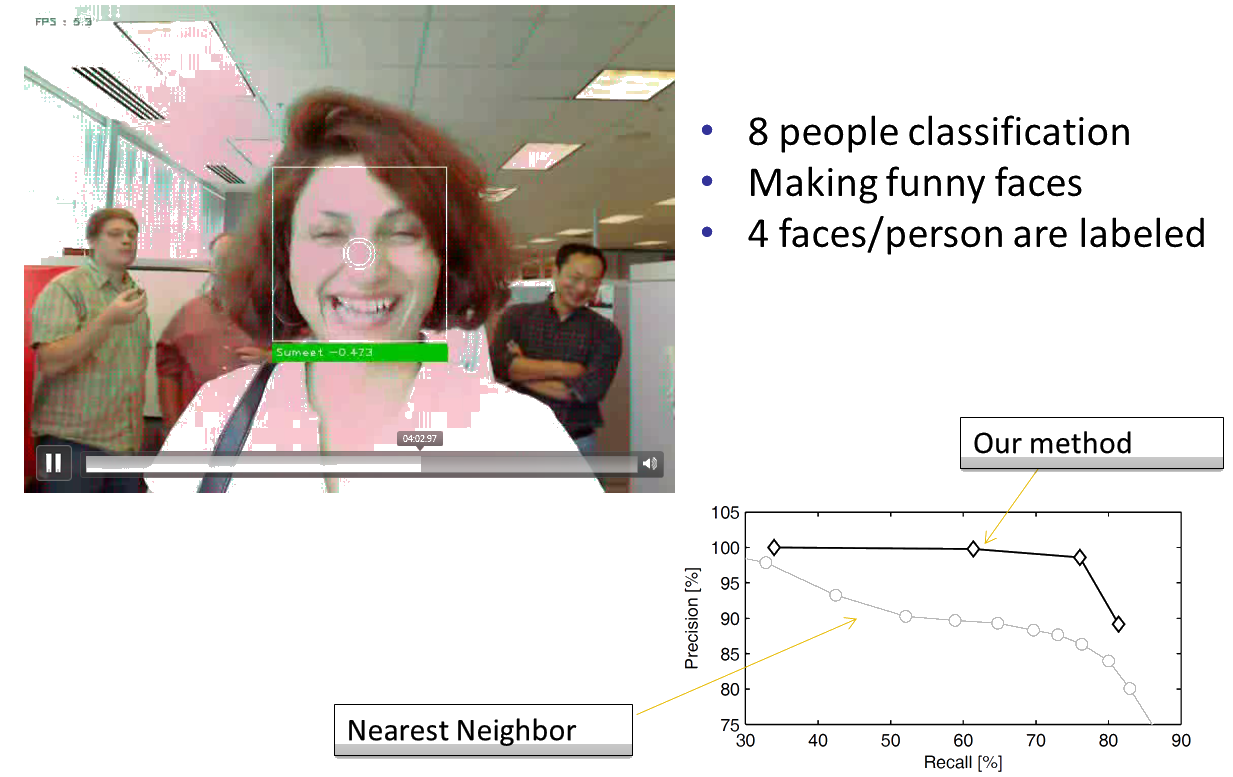
\includegraphics[width=0.85\columnwidth]{../img/b2}
\end{center}

\end{frame}
%%%%%%%%%%%%%%%%%%%%%%%%%%%%%%%%%%%%%%%%%%%%%%%%%%%%%%%%%%%%
%%%%%%%%%%%%%%%%%%%%%%%%%%%%%%%%%%%%%%%%%%%%%%%%%%%%%%%%%%%%



\MakeLastSlide
\end{document}
